
\begin{frame}
\frametitle{Outline} 
\tableofcontents[currentsection]
\end{frame}

\begin{frame}
\frametitle{Gradual typing}\transdissolve<2>
\begin{block}{Principles}
\begin{itemize}
\setlength{\itemsep}{-2pt}
\item Blend statically typed and dynamically typed code
\item Gradual migration instead of converting entire codebase at once
\item Introduce \code{dynamic()} type for type-checking in dynamic typing mode
\end{itemize}
\end{block}

\begin{block}{The \code{dynamic()} type}
\begin{itemize}
\setlength{\itemsep}{-0pt}
\item May turn into any other type at runtime
\item Offers a more relaxed type safety guarantee:\\
 \color<2>{purple}If some program \code{e} has type \code{integer()} and evaluates to a value, \\
      then this value is of type \code{integer()}.
\end{itemize}
\end{block}
\pause\vspace{-4mm}
\begin{exampleblock}{\vspace{-5mm}}
\centering\bf  Same guarantees as \emph{sound gradual typing} but {\color{purple}without inserting
  casts at compilation}
\end{exampleblock}

\end{frame}
%%% def boolean_id(x), do: x
\defverbatim[colored]{\weakApp}{
\begin{minted}{elixir}
id_weak(x_dyn)
# type dynamic()
\end{minted}
}
\defverbatim[colored]{\strongApp}{
\begin{minted}{elixir}
id_weak(x_dyn)                    id_strong(x_dyn)
# type dynamic()                  # type integer() 
\end{minted}
}
\defverbatim[colored]{\strongAppPropagation}{
\begin{minted}{elixir}
id_weak(x_dyn)                    id_strong(x_dyn)
# type dynamic()                  # type integer() !\color{magenta}and dynamic()!
\end{minted}
}

\begin{frame}
\frametitle{Gradual Typing Conundrum}
\textbf{\color{darkslateblue}Typing every expression by \code{dynamic()} is trivially sound \ldots but hardly useful.}

\bigskip
\pause
The system must fulfill two opposite requirements
\begin{enumerate}
	\item it must use \code{dynamic()}  as little as possible so as to be useful, and
	\item it must use \code{dynamic()} enough so as not to hinder the versatility of
	      gradual typing
\end{enumerate}


\bigskip
\pause
The first requirement is fulfilled by the typing of \textbf{\color{darkslateblue}strong functions}, which leverage the run-time checks written by the programmer, or performed by the VM\\[3mm]
The second requirement is fulfilled by the \textbf{\color{darkslateblue}propagation of \code{dynamic()}}.
\end{frame}

\subsection{Strong function types}

\begin{frame}[fragile]{Strong function types}\transdissolve<2,4->
\vspace{-1.5mm}
\begin{block}{(Weak) function type}
\begin{minted}[escapeinside=!!]{elixir}
!\spec! integer() -> integer()
def id_weak(x), do: x !\label{c1}!
\end{minted}
\end{block}
\vspace{-1.6mm}
\pause
\begin{block}{Let \code{x_dyn} be of type \code{dynamic()}}
\vspace{-4.9mm}
    \begin{overlayarea}{\textwidth}{1.3cm}
        \only<2-3>{\weakApp}
        \only<4-7>{\strongApp}
        \only<8>{\strongAppPropagation}
   \end{overlayarea}
\end{block}
\vspace{-1.5mm}
\pause
\begin{block}{Strong function type \only<6->{\smash{(by the programmer)}}}
\begin{minted}[linenos=false,escapeinside=!!]{elixir}
!\spec! integer() -> integer()
def id_strong(x) when is_integer(x), do: x 
\end{minted}
\end{block}
% \begin{block}{Application}
% \begin{minted}{elixir}
% !\spec! dynamic() -> {dynamic(), integer()}
% def dynamic_fun(x), do: {id_weak(x), id_strong(x)}
% \end{minted}
% \end{block}
\pause\pause\pause\pause
\vspace{-.5mm}
% \frametitle{Strong function types (by the VM)}
\begin{block}{Strong function type (by the VM)}
\begin{minted}[linenos=false,escapeinside=!!]{elixir}
!\spec! integer() -> integer()
def double(x), do: x + x
\end{minted}
\end{block}
% \begin{itemize}
% \item Functions with strong types guarantee correct output or runtime type-check failure
% \item Ensures stronger type safety guarantee without modifying Elixir compilation
% % \item Take into account user type checks
% % \item Allows for propagation of \code{dynamic()} type in certain cases
% \end{itemize}
\only<5,6>{\begin{textblock}{15}(1.3,13.5)
    \textbf{\color{darkslateblue}\large Strong function types guarantee correct output or runtime type-check failure}
\end{textblock}}
\only<9>{\begin{textblock}{5}(0,0)
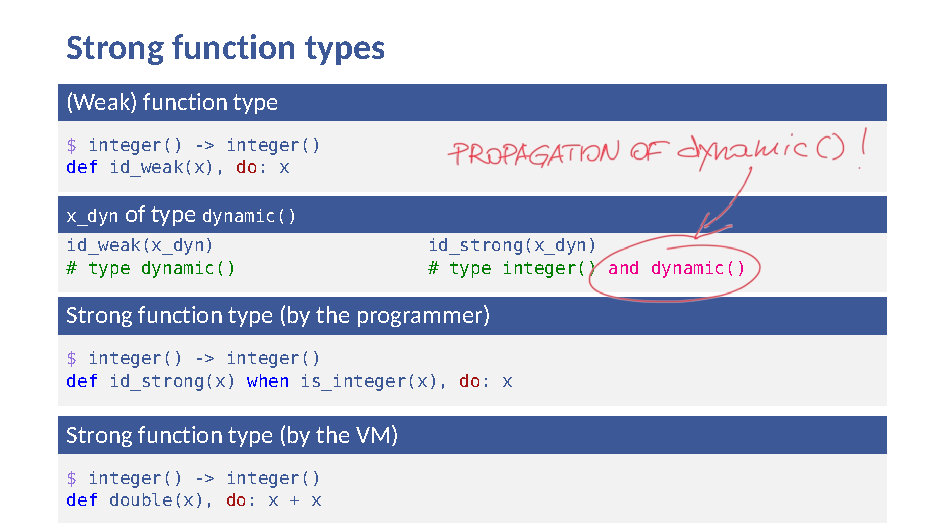
\includegraphics[scale=1]{images/slide-dynprop.pdf}
\end{textblock}}
\end{frame}




\defverbatim[colored]{\dynType}{
\begin{minted}{elixir}
#=> Result type: (integer() or boolean()) !\color{magenta}and dynamic()!
\end{minted}
}
\defverbatim[colored]{\wrongType}{
\begin{minted}{elixir}
#=> Possible type: integer() or boolean()
\end{minted}
}
\defverbatim[colored]{\typeError}{
\begin{minted}{elixir}
#=> Type Error: + undefined for booleans
\end{minted}
}
\defverbatim[colored]{\goodType}{
\begin{minted}{elixir}
#=> Result type: integer()
\end{minted}
}
\defverbatim[colored]{\betterType}{
\begin{minted}{elixir}
#=> Result type: integer() and dynamic()
\end{minted}
}
\defverbatim[colored]{\subtract}{
\begin{minted}{elixir}
def subtract(a, b) do
    a + negate(b)
\end{minted}
}
\defverbatim[colored]{\subtractann}{
\begin{minted}{elixir}
def subtract(a, b) do               !\textcolor{gray}{\footnotesize//if b is given an argument of type dynamic()}!
    a + negate(b)
\end{minted}
}

\subsection{Propagation of \texttt{dynamic()}}

\begin{frame}[fragile]{Propagation of \texttt{dynamic()}}\transdissolve<6>
\textbf{\color{darkslateblue}Apply the (strong function) \code{negate()} function to a \code{dynamic()} argument:}
\vspace{-4mm}
\begin{block}{\vspace{-5mm}}
\begin{minted}{elixir}
!\spec! (integer() -> integer()) and (boolean() -> boolean())
def negate(x) when is_integer(x), do: -x
def negate(x) when is_boolean(x), do: not x
\end{minted}
\vspace{-6.1mm}
\begin{overlayarea}{\textwidth}{2mm}
    \only<2-5>{\wrongType}
    \only<6->{\dynType}
\end{overlayarea}
\hfill
\vspace{1.7mm}
\hfill
\end{block}
\pause\pause\vspace{-6mm}
\begin{block}{\vspace{-6mm}}\vspace{-2mm}
\begin{overlayarea}{\textwidth}{13mm}
\only<3,6>{\subtract}
\only<4,5,7->{\subtractann}
\end{overlayarea}
\vspace{-6.5mm}
\begin{overlayarea}{\textwidth}{2mm}
    \only<5>{\typeError}
    \only<8>{\goodType}
    \only<9->{\betterType}
\end{overlayarea}
\hfill
\vspace{1.7mm}
\end{block}
\pause\pause\pause\pause\pause\pause\pause\vspace{-6mm}
\begin{block}{\vspace{-5mm}}
\begin{minted}{elixir}
def concat(a, b) do
    a ++ negate(b) 
end
#=> Type Error: incompatible types.
\end{minted}
\end{block}
\end{frame}
